\documentclass[twocolumn]{article}
\usepackage[font=small, labelfont=bf]{caption}
\usepackage{sectsty}
\usepackage{dblfloatfix} 
\usepackage{fixltx2e}
\usepackage{graphicx}
\usepackage{color}
\usepackage[letterpaper, margin=0.75in]{geometry}
\usepackage{amsmath}
\usepackage{amsfonts}
\usepackage{tikz}
\usepackage{pgfplots}
\usepackage{parskip}
\usepackage{multicol}
\usepackage{wrapfig}
\usepackage[compact]{titlesec}
\usepackage{float}
\usepackage{pdfpages}
\usepackage{euler}

\begin{document}
\graphicspath{ {Images/} }
\sectionfont{\fontsize{11}{0}\selectfont}
\setlength{\headsep}{0pt}

\titlespacing{\section}{0pt}{*0}{*0}
\titlespacing{\subsection}{0pt}{*0}{*0}
\titlespacing{\subsubsection}{0pt}{*0}{*0}

\setlength{\parindent}{0pt}

\title{Algorithmic Biosynthesis: Staged Glycan Assembly}
\author{Anjali Jaiman and Mukund Thattai}
\maketitle

\section*{Introduction}
O-glycans are a common post-translational modification which attaches a branched oligosaccharide to a serine or threonine amino acid residue on a folded protein. O-glycan biosynthesis is ubiquitous \cite{Apweiler1999} and well-conserved [DATA] across eukaryotes, and yet, sequencing efforts have revealed tremendous structural innovation and diversity. Mammalian o-glycans are composed of a small set of conserved monosaccharides and sugar linkages \cite{Adibekian2010, Herget2008} [Supplemental Fig1], and mainly decorate the extracellular surface of membrane bound and secreted proteins.

O-glycan assembly is processive; a glycosyltransferase shifts a single specific monosaccharide-type from a nucleotide sugar to a particular ``acceptor" monosaccharide on the growing glycan structures, catalyzing a carbon-carbon bond between two particular carbons on the two sugar monomers [Figure 1B]. Thus the minimal specificity of a glycosyltransferase is the acceptor monosaccharide, the donor monosaccharide and the carbon linkage. 

It is possible, and in some cases clear that there are additional specificities [cite]. A glycosyltransferase may have post-node specificity, recognizing additional branches already attached to the acceptor monomer. It may have pre-node specifity, recognizing a pattern of monosaccharides before the acceptor monosaccharide. Or a GTase may have off-node specifity, recognizing a motif on an entirely separate branch of the glycan [Supplemental Figure 1]. These additional specificities can be either activating or inhibitory, and from early and incomplete in vitro studies, many GTases appear to have hierarchical substrate specificity--meaning that they recognize many different substrates with differing strengths--thus as a GTase acts on different substrates, it reacts with different kinetic rates \cite{Blixt2008}. 


But unlike proteins, which are encoded in DNA, glycans are not constructed from a template.

How are the set of glycans structures produced by a cell limited and controlled? Many branched glycan structures, as they are being assembled have more than one acceptor monosaccharide available for glycosylation. Given that many GTases are locally acting and promiscuous, the
web of reactions
forms a complex network which, when drawn out graphically,
indeed resembles a network of diverging and converging paths
leading to a number of different fully-extended N-glycan structures. 


The compartments of the Golgi are not biochemically homogeneous.


microheterogeneity of N-glycans on glycoproteins can
thus be attributed to the nature of the glycosylation reactions and the mixing characteristics of the Golgi apparatus as proteins traverse the system.

\begin{figure*}
    \includegraphics[width=\textwidth]{Figure_1.pdf}
	\caption {A)Schematic comparing different biosynthesis mechanisms: a specialized enzyme contains the exact information needed to catalyze the synthesis of a particular molecule, a metabolite for example; a ribosome uses the mRNA as a template use to ``copy" the information into a peptide; the Golgi apparatus acts as a program, the output of which produces a particular set of glycans. B) GTases transfer a single donor monosaccharide from a nucleotide sugar onto an acceptor monosaccharide on the growing glycan. Most GTases have a minimal specificity of donor, acceptor and carbon pair linkages. Thus, the NeuAc (purple diamond) can be attached to either one of the galactoses (yellow circles). C) Stochasticity inherent in these reactions leads to a diversity of products. D) Competition between enzymes for the same substrate/acceptor monosaccharide also results in a heterogeneous set of structures. E) Polymerization also significantly increases the total set of structures by producing an infinite set of chains containing differing numbers of polymeric repeats. ]}
\end{figure*}


\begin{figure*}
    \includegraphics[width=\textwidth]{Figure_2.pdf}
	\caption{A) Sources of diversity: Incompleteness B) Sources of diversity: Competition. C) Sources of diversity: Polymerization.}
\end{figure*}



\begin{figure*}[h]
    \includegraphics[width=\textwidth]{Figure_3.pdf}
	\caption{A)Entropy as a function of residence time comparing a cyclic reaction network (blue), a cyclic reaction network with a competing tip (red) and a totally ordered reaction network (orange). B) Entropy as a function of average residence time comparing a totally ordered reaction network (orange), a partially ordered reaction network (light blue), and totally ordered reaction network with competition (green).}
\end{figure*}


\begin{figure}[h]
    \includegraphics[width=0.5\textwidth]{Figure_4.pdf}
	\caption{A) Distribution of glycosylation products formed by putting all required locally acting enzymes in each of the three compartments. B) Distribution of glycosylation products when the required enzymes are compartmentalized according to a ``best" partition. C) Distribution of glycosylation products when the average residence times in each compartment of the ``best" partition are not taken as equal. Instead, they are taken 1:5:5. In blue, gillespe simulations were run with total average time is taken at 96.3 for each of the three programs. In mirrored plot (green), the three simulations were run with total average time at 4.8.D) Compares the KL divergences of the three programs above as the distance between a uniform distribution of the four structures and the program distribution as a function of average residence time.}
\end{figure}


\begin{figure*}
    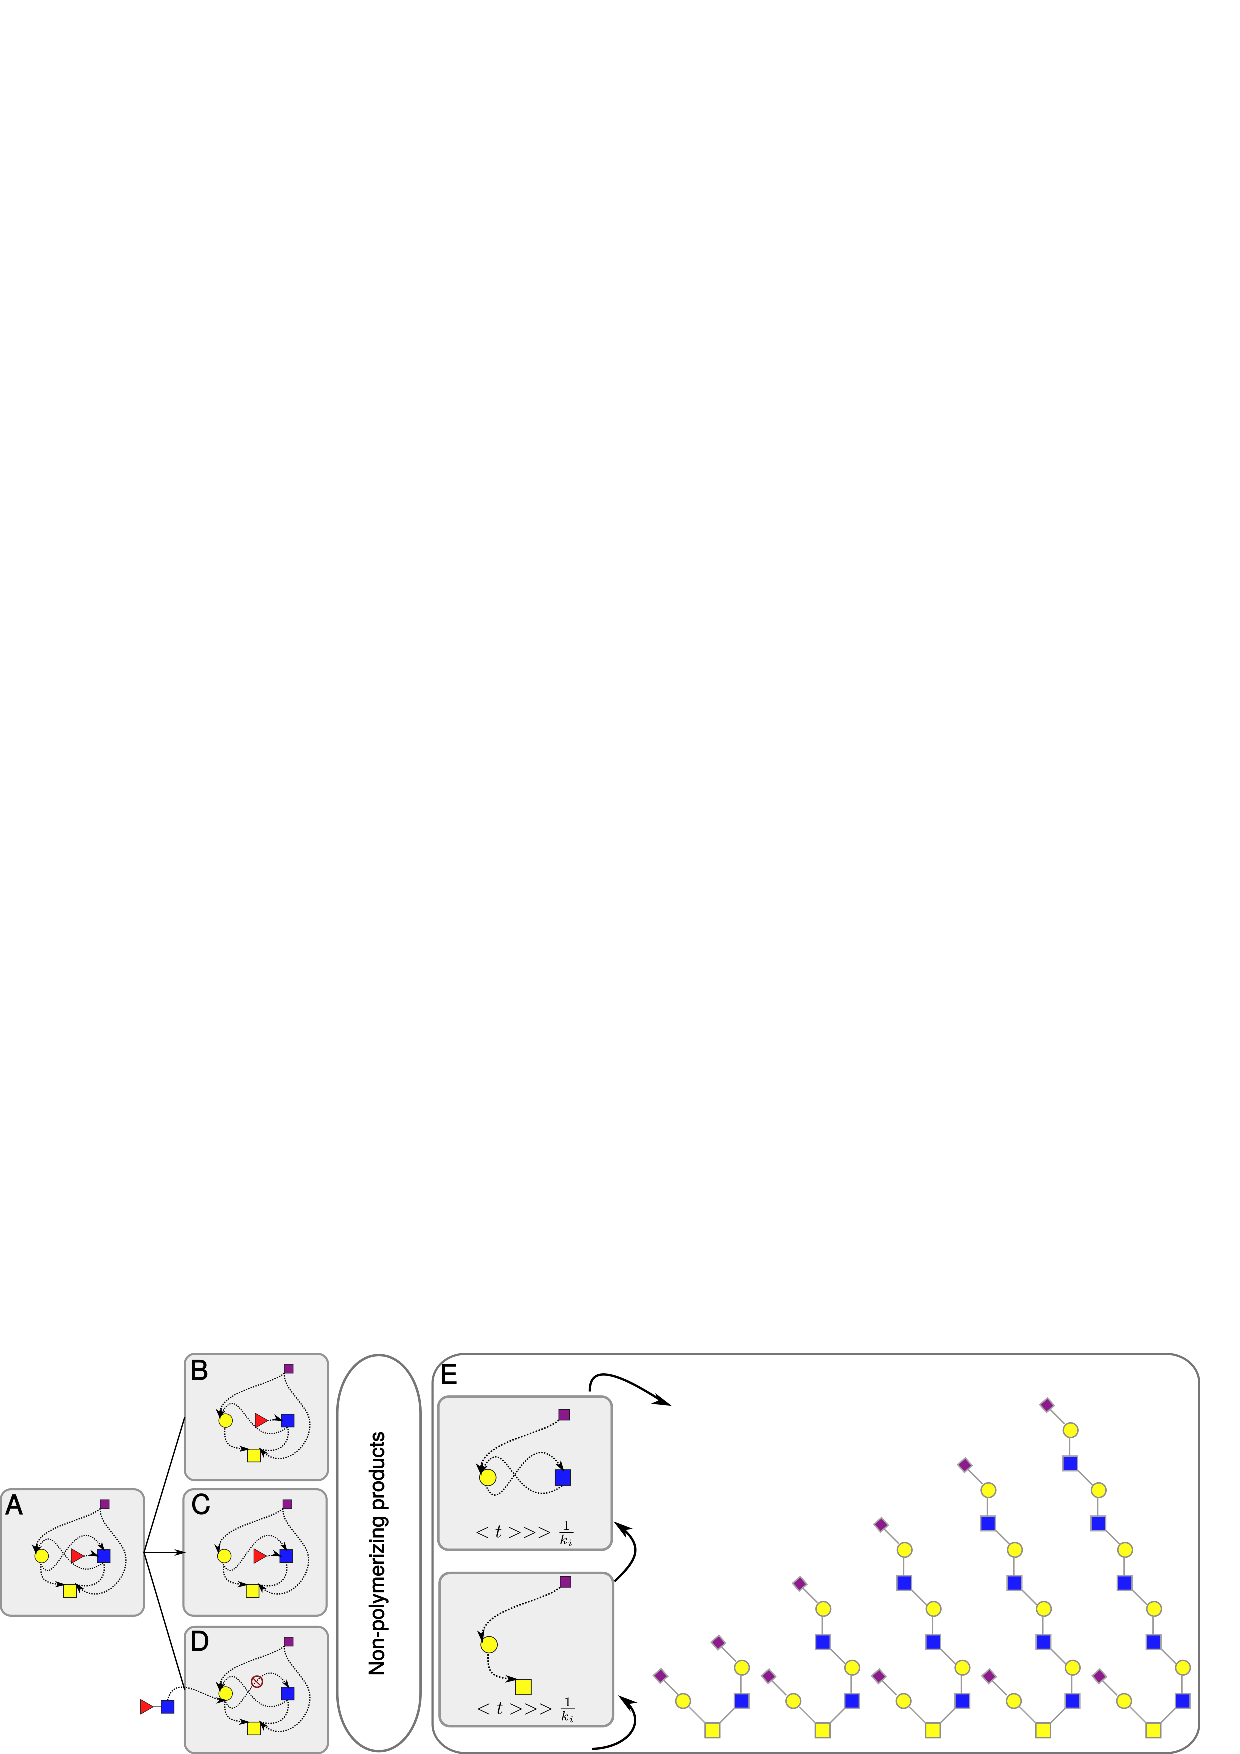
\includegraphics[width=\textwidth]{Figure_6.pdf}
	\caption{A) O-glycans found on equine chorionic gonadotropin \cite{Hokke1994}. O-glycans found on a recombinant MUC1 expressed in B) T47D, C) MDA-MB231, D)ZR-75-1 human breast adenocarcinoma cell lines \cite{Muller2002}. All structure sets contain one or more of the glycan structures found in hCG o-glycan set described above and contain a subset of the linkages found. They are ordered left to right (or top to bottom) in terms of greatest to lowest yields. Trace amounts of other species reported by \cite{Muller2002} were not included.}
\end{figure*}

Usefulness: 


\bibliographystyle{plain}
\bibliography{Glycan_Paper} 

\end{document}


Measuring GTase kinetics and specificities in vivo is a challenge, making it  difficult to reconstruct network topologies or accurately predict of the observable glycan display from a cell's GTase expression profile. But biologists have taken many guesses at how a cell achieves O-glycan reproducibility. Some have argued for a strict ordering of glycan action through highly specific GTases, like those involved in N-glycan synthesis \textbf{[citations]}. Others have argued that complex hierarchieral enzyme specificites and relative kinetics can account for observed glycan data. Still others have argued that for molecular machines, in which heterdimers or larger GTase complexes can strictly order the enzymes leading to greater control over the final glycan set.  \footnote{but this doesnt really make sense to prevent wrongly ordered structures, it only speeds up the kinetics of a series reactions, you still cannot localize certain enzymes together ex. copolymerizing enzymes)} There was also the historical idea that enzyme compartmentalization in the Golgi was a plausible mechanism for ordering the structures, which has been for the most part discarded as cell biologists have come to favor the Golgi maturation model. With the exception of the compartmental ordering model, these explanations for glycan reproducibility,  heterogeneity of cell-type specific and disease glycan phenotypes are accounted for by altered GTase kinetics/specificities through genetic and epigenetic changes.


Conversely, it has been difficult to gain insights into glycan biosynthesis from glycan sequence data. Although sequencing techniques and data have been improving, mass spectrometry---the high throughput method---relies on assumptions about monosaccharide types and linkages in order to reconstruct glycan structures, and without enzyme digestion, it is difficult to assign exact branch locations to different mass fragments. Furthermore, accurate quantitative read-outs of glycan species are not easy to get and so there are potentially numerous low-abundance---and therefore unobserved---glycan structures, which makes it difficult to make any predictions about the order or the relative rates of different reactions involved in o-glycan biosynthesis. \textbf{[Make paragraph longer, with one-sentence explanation of mass spec for self-assembly crowd]}

Here, we do not argue against any of the common hypotheses about glycan biosyntheses; many of these mechanisms are probably simulatenously at play. Instead, we try to confront a simple unexplained element of glycomics hype: 
What is it about observed cellular glycan displays that is surprising? 